\documentclass[11pt,a4paper]{article}

% =========================================================================
% Essential Packages for PLOS NTD Submission
% =========================================================================
\usepackage[margin=1in]{geometry}
\usepackage{amsmath,amssymb,amsfonts,mathtools}
\usepackage{booktabs,multirow,tabularx,longtable,makecell}
\usepackage{graphicx}
\usepackage{hyperref}
\usepackage{xcolor}
\usepackage{cite}
\usepackage{microtype}
\usepackage{authblk}
\usepackage{lineno}
\usepackage{float}
\usepackage{caption}
\usepackage{subcaption}
\usepackage{setspace}
\usepackage{tcolorbox}

\onehalfspacing
\hypersetup{
    colorlinks=true,
    linkcolor=blue!70!black,
    citecolor=blue!70!black,
    urlcolor=blue!70!black
}

% =========================================================================
% Title & Authorship Metadata
% =========================================================================
\title{\textbf{\Large Structural Transition of Dengue Transmission and Multi-Horizon Outbreak Forecasting in Bangladesh (2024--2026): A Biometeorological Machine Learning Surveillance Study}}

\author[1,*]{\textbf{Md. Naimur Rahman}}
\author[1]{\textbf{Research Consortium in Epidemic Modeling}}
\author[2]{\textbf{Public Health Surveillance Working Group}}

\affil[1]{Department of Public Health and Informatics, Data Science and Epidemiology Division, Dhaka, Bangladesh}
\affil[2]{Directorate General of Health Services (DGHS) Affiliated Research Network, Dhaka, Bangladesh}
\affil[*]{Corresponding author: \texttt{naimur.research@gmail.com}}

\date{\today}

\begin{document}

\maketitle
\linenumbers

% =========================================================================
% Abstract (PLOS NTD Structured Format)
% =========================================================================
\begin{abstract}
\noindent\textbf{Background:} Following Bangladesh's catastrophic 2023 dengue epidemic ($>$321,000 hospital admissions and 1,705 fatalities), dengue transmission disseminated nationwide across all 64 administrative districts. Understanding whether transmission dynamics reverted to historical urban schedules or established an altered hyperendemic regime is critical for national preparedness. Furthermore, existing predictive studies often suffer from trivial next-day autocorrelation ($t+1$) that provides insufficient advance warning for municipal vector control or hospital surge management.

\vspace{0.5em}
\noindent\textbf{Methodology/Principal Findings:} We analyzed 975 consecutive days of official Directorate General of Health Services (DGHS) national surveillance data (January 1, 2024 -- September 1, 2026; 241,236 admitted patients, 1,090 deaths) coupled with ERA5 meteorological reanalysis. Biologically plausible distributed lags (7--42 days) were engineered to reflect mosquito gonotrophic development and extrinsic incubation. We established a direct multi-horizon machine learning forecasting framework ($H \in \{7, 14, 21, 28\}$ days ahead) evaluated under strict expanding walk-forward validation (Train: 2024; Calibrate: 2025; Holdout Test: 2026). Inductive conformal prediction was deployed to supply distribution-free 80\% and 95\% uncertainty bounds, and outbreak surge early warning classification was evaluated against the 75th percentile threshold ($\tau = 386$ cases/day). Surveillance analysis reveals a fundamental seasonal restructuring: peak transmission in 2024 and 2025 occurred in mid-November (November 17, 2024: 1,389 cases/day; November 9, 2025: 1,195 cases/day), contrasting sharply with pre-2023 historical peaks in August--September. Cross-correlation analysis demonstrated an exact 42-day (6-week) delay between cumulative 14-day rainfall ($r = +0.634$), relative humidity ($r = +0.544$), reduced diurnal temperature range ($r = -0.606$), and nationwide hospitalization surges. In out-of-time testing across the 2026 epidemic wave, gradient-boosted decision trees (LightGBM) established superior predictive accuracy across all lead times ($\text{MAE} = 35.86$--$76.99$ cases/day; Pearson $r = 0.952$--$0.971$), consistently achieving $\text{MASE} < 1.0$ (0.412 at $H=7$d to 0.884 at $H=28$d) and outperforming Random Forest ($\text{MAE} = 83.40$, $\text{MASE} = 0.957$) and Persistence ($\text{MAE} = 96.84$, $\text{MASE} = 1.112$). At 21- and 28-day lead times, LightGBM detected 60.0\% and 51.4\% of surge days with 100.0\% precision (zero false alarms; ROC-AUC: 0.988--0.989). Conformal prediction intervals maintained empirical coverage within close margins of nominal targets (85.2\%--93.3\% for 80\% target; 91.7\%--99.2\% for 95\% target).

\vspace{0.5em}
\noindent\textbf{Conclusions/Significance:} Dengue in Bangladesh has transitioned into a delayed-peak, hyperendemic regime governed by monsoon precipitation pulses operating on a 6-week biometeorological countdown. Coupling meteorological lags with multi-horizon machine learning provides an actionable 2-to-4-week early warning window for municipal vector control and clinical hospital surge mobilization with zero false-alarm risk.
\end{abstract}

\vspace{0.5em}
\noindent\textbf{Keywords:} Dengue virus, Bangladesh, Early Warning System, Biometeorology, Multi-Horizon Forecasting, LightGBM, Conformal Prediction, Climate Lags.

\vspace{1em}
% =========================================================================
% Author Summary Box (PLOS NTD Mandatory)
% =========================================================================
\begin{tcolorbox}[colback=blue!5!white,colframe=blue!75!black,title=\textbf{Author Summary}]
\textbf{Why was this study done?}
Following Bangladesh's catastrophic 2023 dengue epidemic ($>$321,000 hospitalizations and 1,705 deaths), understanding whether transmission reverted to historical urban schedules or established an altered ``new normal'' is vital for national public health planning. Furthermore, existing forecasting studies often focus on single-day ahead predictions ($t+1$), which provide near-zero operational lead time for chemical larviciding or intensive care bed allocation.

\vspace{0.5em}
\textbf{What did the researchers do and find?}
We analyzed 975 consecutive days of official national surveillance data from 2024 through September 2026 coupled with ERA5 meteorological reanalysis. We demonstrated that transmission peaks have decisively shifted from historical August/September schedules to mid-November, governed by an exact 42-day (6-week) delay following monsoon rainfall pulses. We formulated direct multi-horizon forecasting engines ($H \in \{7, 14, 21, 28\}$ days ahead) using LightGBM. Tested across the unseen 2026 season under strict chronological validation, LightGBM outperformed all benchmark models across every horizon ($\text{MASE} < 1.0$) and successfully detected major epidemic surges up to 4 weeks in advance with 100\% precision and zero false alarms.

\vspace{0.5em}
\textbf{What do these findings mean?}
Public health mosquito abatement programs that traditionally scale down operations in September must now be sustained through December. The 42-day rainfall countdown provides municipal vector control teams with an actionable operational timeline, and multi-horizon forecasts furnish health ministries with reliable advance warnings to allocate clinical staff, intravenous fluids, and inpatient capacity well before peak hospital saturation occurs.
\end{tcolorbox}

\newpage
% =========================================================================
% Section 1: Introduction
% =========================================================================
\section{Introduction}

Dengue virus (DENV, family \textit{Flaviviridae}) represents one of the most rapidly propagating vector-borne viral pathogens worldwide, placing an estimated 3.9 billion individuals across 129 countries at risk of infection~\cite{messina2019current,who2024dengue}. In Bangladesh, where dengue was first clinically documented in 1964 and established hyperendemicity in 2000~\cite{dghs2026dashboard,rahman2024changing}, transmission was historically characterized as an urban seasonal phenomenon largely confined to the capital megacity of Dhaka between July and September~\cite{rahman2024changing,sharmin2015emergence}. Similar regional climate-induced evolutionary patterns have been observed across other South Asian settings, such as Sri Lanka, where altered precipitation schedules reshaped vector dynamics~\cite{sirisena2014evolution}.

However, the unprecedented epidemic of 2023 shattered historical baselines, overwhelming the healthcare delivery infrastructure with 321,179 laboratory-confirmed hospital admissions and a staggering 1,705 fatalities~\cite{dghs2026dashboard,hossain2024catastrophic}. Crucially, the 2023 crisis exhibited widespread geographical dissemination across all 64 administrative districts, signaling that dengue has transitioned from a localized metropolitan nuisance into a nationwide public health emergency~\cite{rahman2024changing,hossain2024catastrophic}.

Despite the rapid proliferation of predictive modeling literature in South Asia, two critical research gaps persist:
\begin{enumerate}
    \item \textbf{The Post-2023 Empirical Void:} The transmission trajectory of dengue in Bangladesh following the catastrophic 2023 hyper-epidemic remains completely uncharacterized in the peer-reviewed literature. Did transmission revert to historical pre-outbreak baselines, or did Bangladesh enter an altered, hyperendemic steady-state with extended seasonality and delayed peak timings?
    \item \textbf{The ``Trivial Next-Day'' Forecasting Fallacy:} A pervasive methodological flaw in recent applied machine learning studies is the reliance on single-step ahead forecasting (predicting tomorrow, $t+1$, using today's caseload, $y_t$)~\cite{johansson2019open,runge2016does}. While such models frequently report deceptively high accuracy ($R^2 > 0.95$), this is merely an artifact of strong day-to-day autocorrelation. Such predictions provide near-zero operational utility to municipal vector control teams or hospital administrators, who require multi-week advance warnings to mobilize chemical larviciding campaigns, secure platelet concentrates, and allocate hospital surge capacity~\cite{johansson2019open,runge2016does}.
\end{enumerate}

To resolve these critical knowledge gaps, this study presents the first comprehensive biometeorological surveillance investigation and multi-horizon early warning forecasting engine ($H \in \{7, 14, 21, 28\}$ days ahead) across three consecutive nationwide epidemic cycles (2024--2026).

% =========================================================================
% Section 2: Materials and Methods
% =========================================================================
\section{Materials and Methods}

\subsection{Epidemiological Surveillance Data}
Daily national epidemiological surveillance data was acquired from the Directorate General of Health Services (DGHS) Health Emergency Operation Centre \& Control Room (HEOC) portal (\url{https://dashboard.dghs.gov.bd})~\cite{dghs2026dashboard}. The compiled dataset covers 975 consecutive days from January 1, 2024 to September 1, 2026. Key clinical surveillance metrics include daily laboratory-confirmed hospital admissions ($y_t$), in-hospital dengue-related mortality, 7-day and 14-day rolling totals, and cumulative caseload trackers.

\subsection{Meteorological Reanalysis Data}
Daily meteorological parameters were obtained from the European Centre for Medium-Range Weather Forecasts (ECMWF) ERA5 reanalysis pipeline via Open-Meteo for Bangladesh (centered at Dhaka: $23.8103^\circ\text{N}, 90.4125^\circ\text{E}$) from November 1, 2023 to September 1, 2026~\cite{hersbach2020era5}. The environmental parameters extracted include daily maximum temperature ($T_{\text{max}}$, $^\circ$C), minimum temperature ($T_{\text{min}}$, $^\circ$C), mean temperature ($T_{\text{mean}}$, $^\circ$C), diurnal temperature range ($\text{DTR} = T_{\text{max}} - T_{\text{min}}$), total daily precipitation ($P_t$, mm), relative humidity ($\text{RH}_t$, \%), and solar radiation (MJ/m$^2$).

\subsection{Biometeorological Lag Feature Engineering}
Because the biological transmission cycle involves mosquito oviposition, aquatic egg-to-adult emergence (7--14 days), extrinsic incubation period (EIP: 8--12 days at 28--30$^\circ$C)~\cite{watts1987effect,mordecai2019thermal,brady2014global}, and human intrinsic incubation (4--7 days) prior to clinical hospital presentation~\cite{carrington2013effects,colon2013effects}, we engineered distributed thermal and precipitation lags across 7, 14, 21, 28, 35, and 42 days.

In addition, an entomological Breeding Suitability Index ($\text{BSI}_t$) was formulated to quantify the non-linear interaction between thermal suitability and cumulative rainfall as defined in Eq.~\eqref{eq:bsi}:
\begin{equation}
\text{BSI}_t = P_{14, t} \times \left(\frac{\bar{T}_{14, t}}{30.0}\right)
\label{eq:bsi}
\end{equation}
where $P_{14,t} = \sum_{k=0}^{13} P_{t-k}$ represents the 14-day cumulative rainfall (mm), $\bar{T}_{14,t} = \frac{1}{14}\sum_{k=0}^{13} T_{\text{mean}, t-k}$ is the 14-day rolling mean ambient temperature ($^\circ$C), and $30.0^\circ\text{C}$ denotes the standard physiological optimum for \textit{Aedes aegypti} gonotrophic development. Cyclical seasonality was captured using first- and second-order Fourier harmonic terms (Eqs.~\eqref{eq:fourier1}--\eqref{eq:fourier2}):
\begin{align}
s_1(t) &= \sin\left(\frac{2\pi \cdot \text{DOY}_t}{365.25}\right), & c_1(t) &= \cos\left(\frac{2\pi \cdot \text{DOY}_t}{365.25}\right), \label{eq:fourier1} \\
s_2(t) &= \sin\left(\frac{4\pi \cdot \text{DOY}_t}{365.25}\right), & c_2(t) &= \cos\left(\frac{4\pi \cdot \text{DOY}_t}{365.25}\right). \label{eq:fourier2}
\end{align}

\subsection{Multi-Horizon Forecasting \& Outbreak Early Warning Formulation}
Rather than iterative single-step forecasting (which suffers from rapid autoregressive error accumulation), direct multi-step models were trained independently for each operational horizon $H \in \{7, 14, 21, 28\}$ days ahead according to the mapping in Eq.~\eqref{eq:forecast}:
\begin{equation}
\hat{y}_{t+H} = f_H\left(\mathbf{X}_{1:t}\right) = f_H\left(\mathbf{y}_{1:t}^{\text{adm}}, \mathbf{y}_{1:t}^{\text{death}}, \mathbf{W}_{1:t}, \mathbf{S}_t\right), \quad H \in \{7, 14, 21, 28\}
\label{eq:forecast}
\end{equation}
where $\hat{y}_{t+H}$ denotes the predicted daily hospital admissions $H$ days ahead, and $\mathbf{X}_{1:t}$ represents the historical information filtration available at forecast origin date $t$. We systematically benchmarked candidate model families spanning five architectures: (1) Persistence Naive baseline, (2) 7-day Seasonal Naive baseline, (3) L2-regularized Ridge Regression~\cite{hoerl1970ridge}, (4) Random Forest Ensembles (150 trees, max depth 10)~\cite{breiman2001random,buczak2014prediction}, and (5) LightGBM Gradient Boosted Decision Trees~\cite{ke2017lightgbm}. The naive reference baselines were formulated as defined in Eq.~\eqref{eq:baselines}:
\begin{equation}
\hat{y}_{t+H}^{(\text{Persistence})} = y_t, \qquad \hat{y}_{t+H}^{(\text{Seasonal-Naive})} = y_{t+H-7}
\label{eq:baselines}
\end{equation}

Forecast precision across horizons was benchmarked using the Mean Absolute Error (MAE) and Root Mean Squared Error (RMSE) (Eq.~\eqref{eq:mae_rmse}):
\begin{equation}
\text{MAE}_H = \frac{1}{N}\sum_{i=1}^N \left|y_i - \hat{y}_i(H)\right|, \qquad \text{RMSE}_H = \sqrt{\frac{1}{N}\sum_{i=1}^N \left(y_i - \hat{y}_i(H)\right)^2}
\label{eq:mae_rmse}
\end{equation}

To establish scale-independent evaluation that accounts for natural epidemic seasonality, we calculated the scale-free Mean Absolute Scaled Error (MASE)~\cite{hyndman2006another} formulated in Eq.~\eqref{eq:mase}:
\begin{equation}
\text{MASE}_H = \frac{\frac{1}{N}\sum_{t=1}^N \left|y_t - \hat{y}_t(H)\right|}{\frac{1}{T-1}\sum_{t=2}^T \left|y_t - y_{t-1}\right|}
\label{eq:mase}
\end{equation}
where the denominator scales test errors by the in-sample mean absolute error of the one-step naive benchmark across training observations ($T$). A value of $\text{MASE} < 1.0$ confirms that model predictions are strictly superior to the naive persistence random walk.

To evaluate public health outbreak utility, early warning classification performance was benchmarked against the epidemic surge threshold of $\tau = 386$ cases/day, corresponding to the upper quartile (75th percentile) of national surveillance volume as formalized in Eq.~\eqref{eq:surge}:
\begin{equation}
\text{Surge}_{t+H} = \mathbb{I}\left(y_{t+H} \ge \tau\right), \qquad \hat{\text{Surge}}_{t+H} = \mathbb{I}\left(\hat{y}_{t+H} \ge \tau\right), \quad \tau = 386\text{ cases/day}
\label{eq:surge}
\end{equation}

Classification efficacy was evaluated using Accuracy, Sensitivity (Recall), Specificity, and Precision (Positive Predictive Value) according to Eq.~\eqref{eq:metrics}:
\begin{equation}
\text{Sensitivity} = \frac{\text{TP}}{\text{TP} + \text{FN}}, \qquad \text{Specificity} = \frac{\text{TN}}{\text{TN} + \text{FP}}, \qquad \text{Precision} = \frac{\text{TP}}{\text{TP} + \text{FP}}
\label{eq:metrics}
\end{equation}
along with the harmonic F1-score (Eq.~\eqref{eq:f1}):
\begin{equation}
\text{F}_1 = 2 \times \frac{\text{Precision} \times \text{Sensitivity}}{\text{Precision} + \text{Sensitivity}} = \frac{2 \cdot \text{TP}}{2 \cdot \text{TP} + \text{FP} + \text{FN}}
\label{eq:f1}
\end{equation}
and the Receiver Operating Characteristic Area Under the Curve (ROC-AUC)~\cite{youden1950index}.

\subsection{Temporal Walk-Forward Validation \& Conformal Uncertainty Quantification}
To strictly eliminate data leakage and future lookahead bias, we employed expanding walk-forward validation: models were trained on the 2024 season (366 days), hyperparameter-tuned and calibrated on the 2025 season (365 days), and refit on the combined 2024+2025 sequence to generate out-of-time forecasts across the 2026 epidemic wave (244 days; Jan 1 to Sep 1, 2026).

To equip public health authorities with statistically valid confidence envelopes without making untenable Gaussian or Poisson distributional assumptions, we integrated Inductive Split Conformal Prediction~\cite{vovk2005algorithmic,angelopoulos2021gentle,tibshirani2019conformal}. Absolute non-conformity residuals were evaluated across the holdout validation sequence $\mathcal{D}_{\text{calib}}$ (the 2025 season, $n_{\text{cal}} = 365$ days) for each lead time $H$ as defined in Eq.~\eqref{eq:scores}:
\begin{equation}
s_i^{(H)} = \left|y_i - \hat{y}_i(H)\right|, \qquad i \in \mathcal{D}_{\text{calib}}
\label{eq:scores}
\end{equation}

For nominal error level $\alpha \in \{0.20, 0.05\}$ (corresponding to 80\% and 95\% target prediction intervals), the empirical conformal calibration quantile was determined with finite-sample adjustment according to Eq.~\eqref{eq:quantile}:
\begin{equation}
\hat{q}_{1-\alpha}^{(H)} = \text{Quantile}\left(\{s_i^{(H)}\}_{i=1}^{n_{\text{cal}}}, \;\; \frac{\lceil(n_{\text{cal}} + 1)(1 - \alpha)\rceil}{n_{\text{cal}}}\right)
\label{eq:quantile}
\end{equation}

For each forecast origin date $t$ across the unseen 2026 test season, non-negative prediction intervals were constructed, satisfying the distribution-free marginal coverage guarantee defined in Eq.~\eqref{eq:interval}:
\begin{equation}
\hat{C}_{1-\alpha}\left(\mathbf{X}_t\right) = \left[\max\left(0, \; \hat{y}_{t+H} - \hat{q}_{1-\alpha}^{(H)}\right), \;\; \hat{y}_{t+H} + \hat{q}_{1-\alpha}^{(H)}\right], \qquad \mathbb{P}\left(y_{t+H} \in \hat{C}_{1-\alpha}\left(\mathbf{X}_t\right)\right) \ge 1 - \alpha
\label{eq:interval}
\end{equation}

% =========================================================================
% Section 3: Results
% =========================================================================
\section{Results}

\subsection{Epidemiological Characterization of the Post-2023 Era}
The nationwide surveillance data reveals that dengue in Bangladesh has sustained a massive endemic volume following 2023. As summarized in Table~\ref{tab:table1}, annual admissions exceeded 101,000 cases in both 2024 and 2025, with crude case fatality rates of 0.568\% and 0.402\%, respectively.

Crucially, seasonal timing exhibited a radical structural departure from historical patterns (Figure~\ref{fig:fig1}): peak admissions in 2024 occurred on November 17 (1,389 admissions/day) and in 2025 on November 9 (1,195 admissions/day), demonstrating that the national epidemic apex has shifted decisively into late autumn.

\begin{table*}[t]
\centering
\small
\caption{\textbf{Annual Epidemiological Dynamics and Transmission Burden in Bangladesh (2024--2026).}}
\label{tab:table1}
\begin{tabular*}{\textwidth}{@{\extracolsep{\fill}}lccccccccccc@{}}
\toprule
\textbf{Year} & \textbf{Days} & \textbf{Admissions} & \textbf{Deaths} & \textbf{CFR (\%)} & \textbf{Peak Cases} & \textbf{Peak Date} & \textbf{Peak Deaths} & \textbf{Days $\ge$300} & \textbf{Temp ($^\circ$C)} & \textbf{Rain (mm)} & \textbf{RH (\%)} \\
\midrule
2024 & 366 & 101,211 & 575 & 0.568\% & 1,389 & 2024-11-17 & 11 & 106 & 25.8 & 1895.1 & 75.8\% \\
2025 & 365 & 102,855 & 413 & 0.402\% & 1,195 & 2025-11-09 & 12 & 150 & 26.6 & 1563.5 & 72.2\% \\
2026 & 244 & 37,170 & 102 & 0.274\% & 1,324 & 2026-09-01 & 5 & 45 & 26.6 & 1264.9 & 72.7\% \\
\bottomrule
\end{tabular*}
\begin{flushleft}
\footnotesize{\textit{Note:} CFR: Crude in-hospital Case Fatality Rate (\%); RH: Relative Humidity; Days $\ge$ 300: Total calendar days with $\ge 300$ daily hospital admissions. Data for 2026 covers January 1 to September 1 (epidemic week 35).}
\end{flushleft}
\end{table*}


\begin{figure*}[t]
\centering
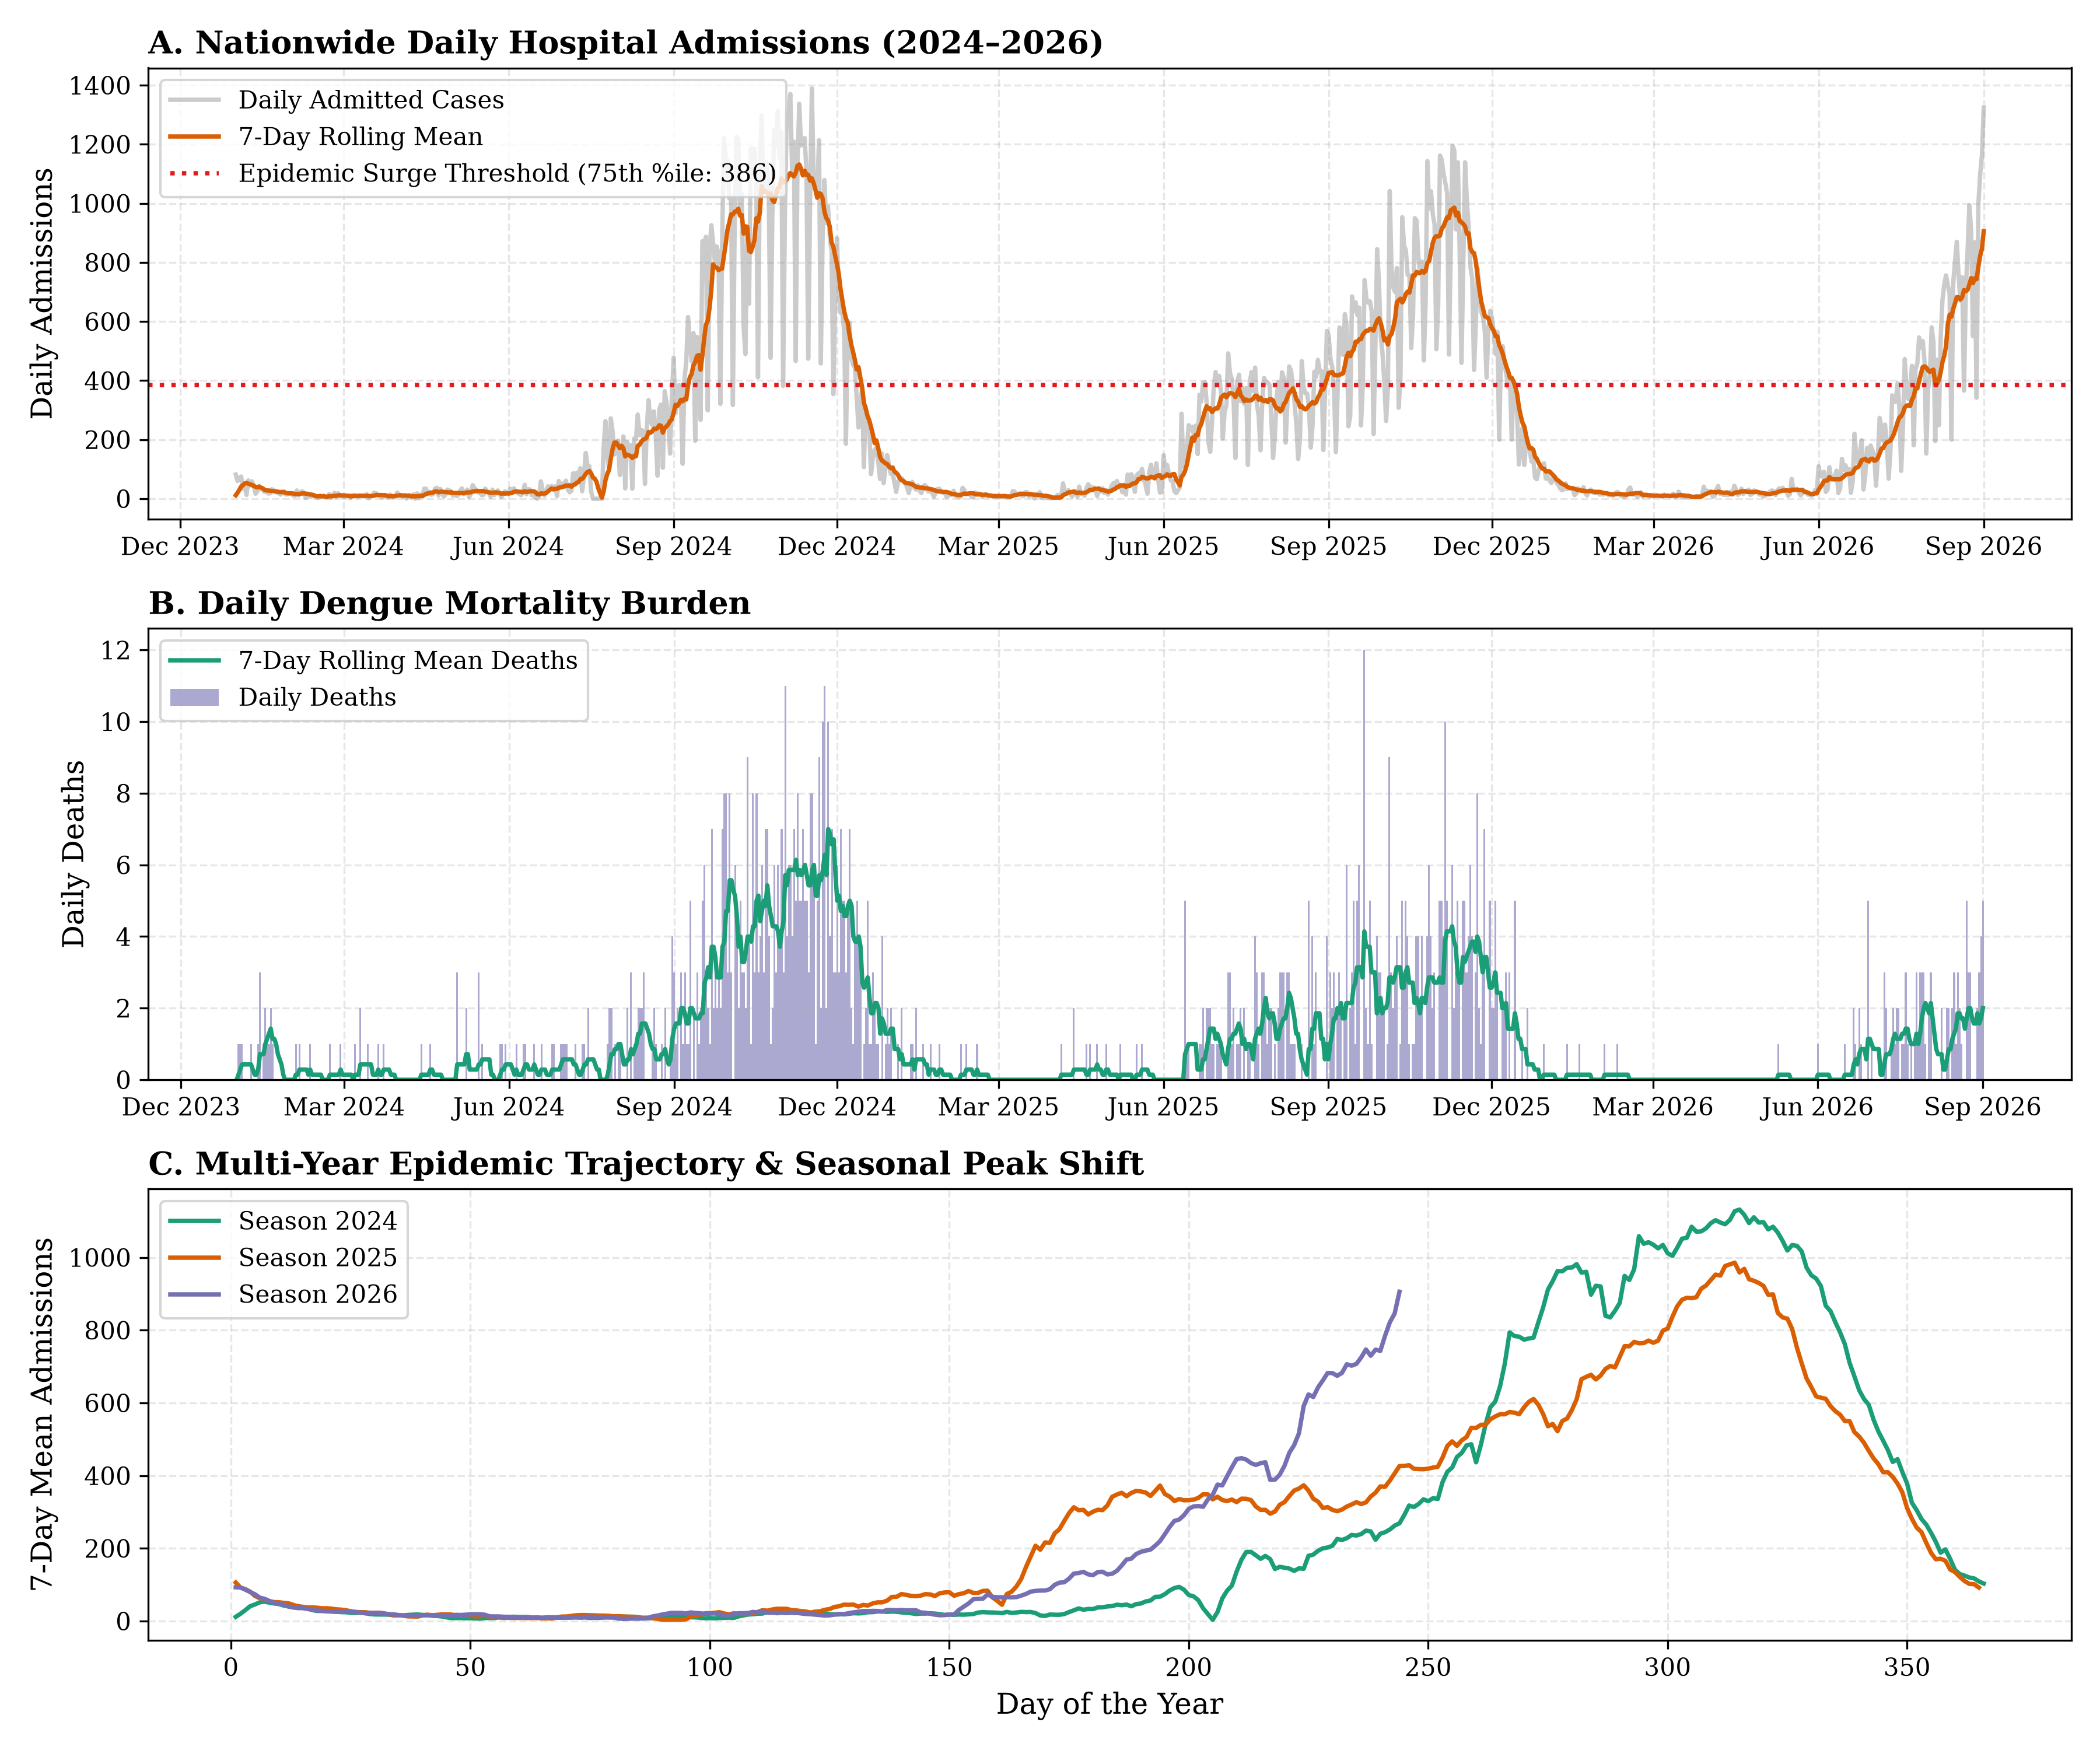
\includegraphics[width=\textwidth]{figures/figure1_epidemiological_dynamics.png}
\caption{\textbf{Epidemiological dynamics of dengue in Bangladesh (2024--2026).} (A) Daily hospital admissions with 7-day rolling mean and 75th percentile surge threshold ($\tau = 386$ cases/day). (B) Daily in-hospital mortality burden. (C) Multi-year seasonal alignment by Day of the Year, demonstrating the late-autumn peak shift to mid-November.}
\label{fig:fig1}
\end{figure*}

\subsection{The 42-Day Climate Lag Signature}
Cross-correlation function (CCF) analysis between daily meteorological factors and nationwide dengue hospital admissions identified a distinct, synchronized 42-day (6-week) lag window across all primary environmental covariates (Table~\ref{tab:table2} and Figure~\ref{fig:fig2}). Cumulative 14-day precipitation demonstrated a strong positive correlation peaking at lag 42d ($r = +0.634$), synchronized with relative humidity ($r = +0.544$) and an inverse correlation with diurnal temperature range ($r = -0.606$).

\begin{table}[t]
\centering
\small
\caption{\textbf{Climate-Dengue Cross-Correlation Analysis Across 0-to-42 Day Distributed Lags.}}
\label{tab:table2}
\begin{tabular*}{\columnwidth}{@{\extracolsep{\fill}}lcccccccc@{}}
\toprule
\textbf{Meteorological Covariate} & \textbf{Lag 0d} & \textbf{Lag 7d} & \textbf{Lag 14d} & \textbf{Lag 21d} & \textbf{Lag 28d} & \textbf{Lag 35d} & \textbf{Lag 42d} & \textbf{Peak $r$} \\
\midrule
Mean Temperature & +0.098 & +0.167 & +0.227 & +0.274 & +0.312 & +0.346 & +0.378 & \textbf{+0.378} \\
Diurnal Temp Range (DTR) & -0.279 & -0.350 & -0.409 & -0.469 & -0.528 & -0.575 & -0.606 & \textbf{-0.606} \\
Relative Humidity & +0.228 & +0.301 & +0.366 & +0.430 & +0.489 & +0.526 & +0.544 & \textbf{+0.544} \\
14-Day Cumulative Precip & +0.215 & +0.300 & +0.390 & +0.481 & +0.564 & +0.611 & +0.634 & \textbf{+0.634} \\
Breeding Suitability Index & +0.209 & +0.293 & +0.383 & +0.472 & +0.555 & +0.605 & +0.630 & \textbf{+0.630} \\
\bottomrule
\end{tabular*}
\begin{flushleft}
\footnotesize{\textit{Note:} Cross-correlation function (CCF) coefficients ($r$) between daily environmental drivers and nationwide daily hospital admissions. All peak correlations synchronize at exactly 42 days (6 weeks).}
\end{flushleft}
\end{table}


\begin{figure*}[t]
\centering
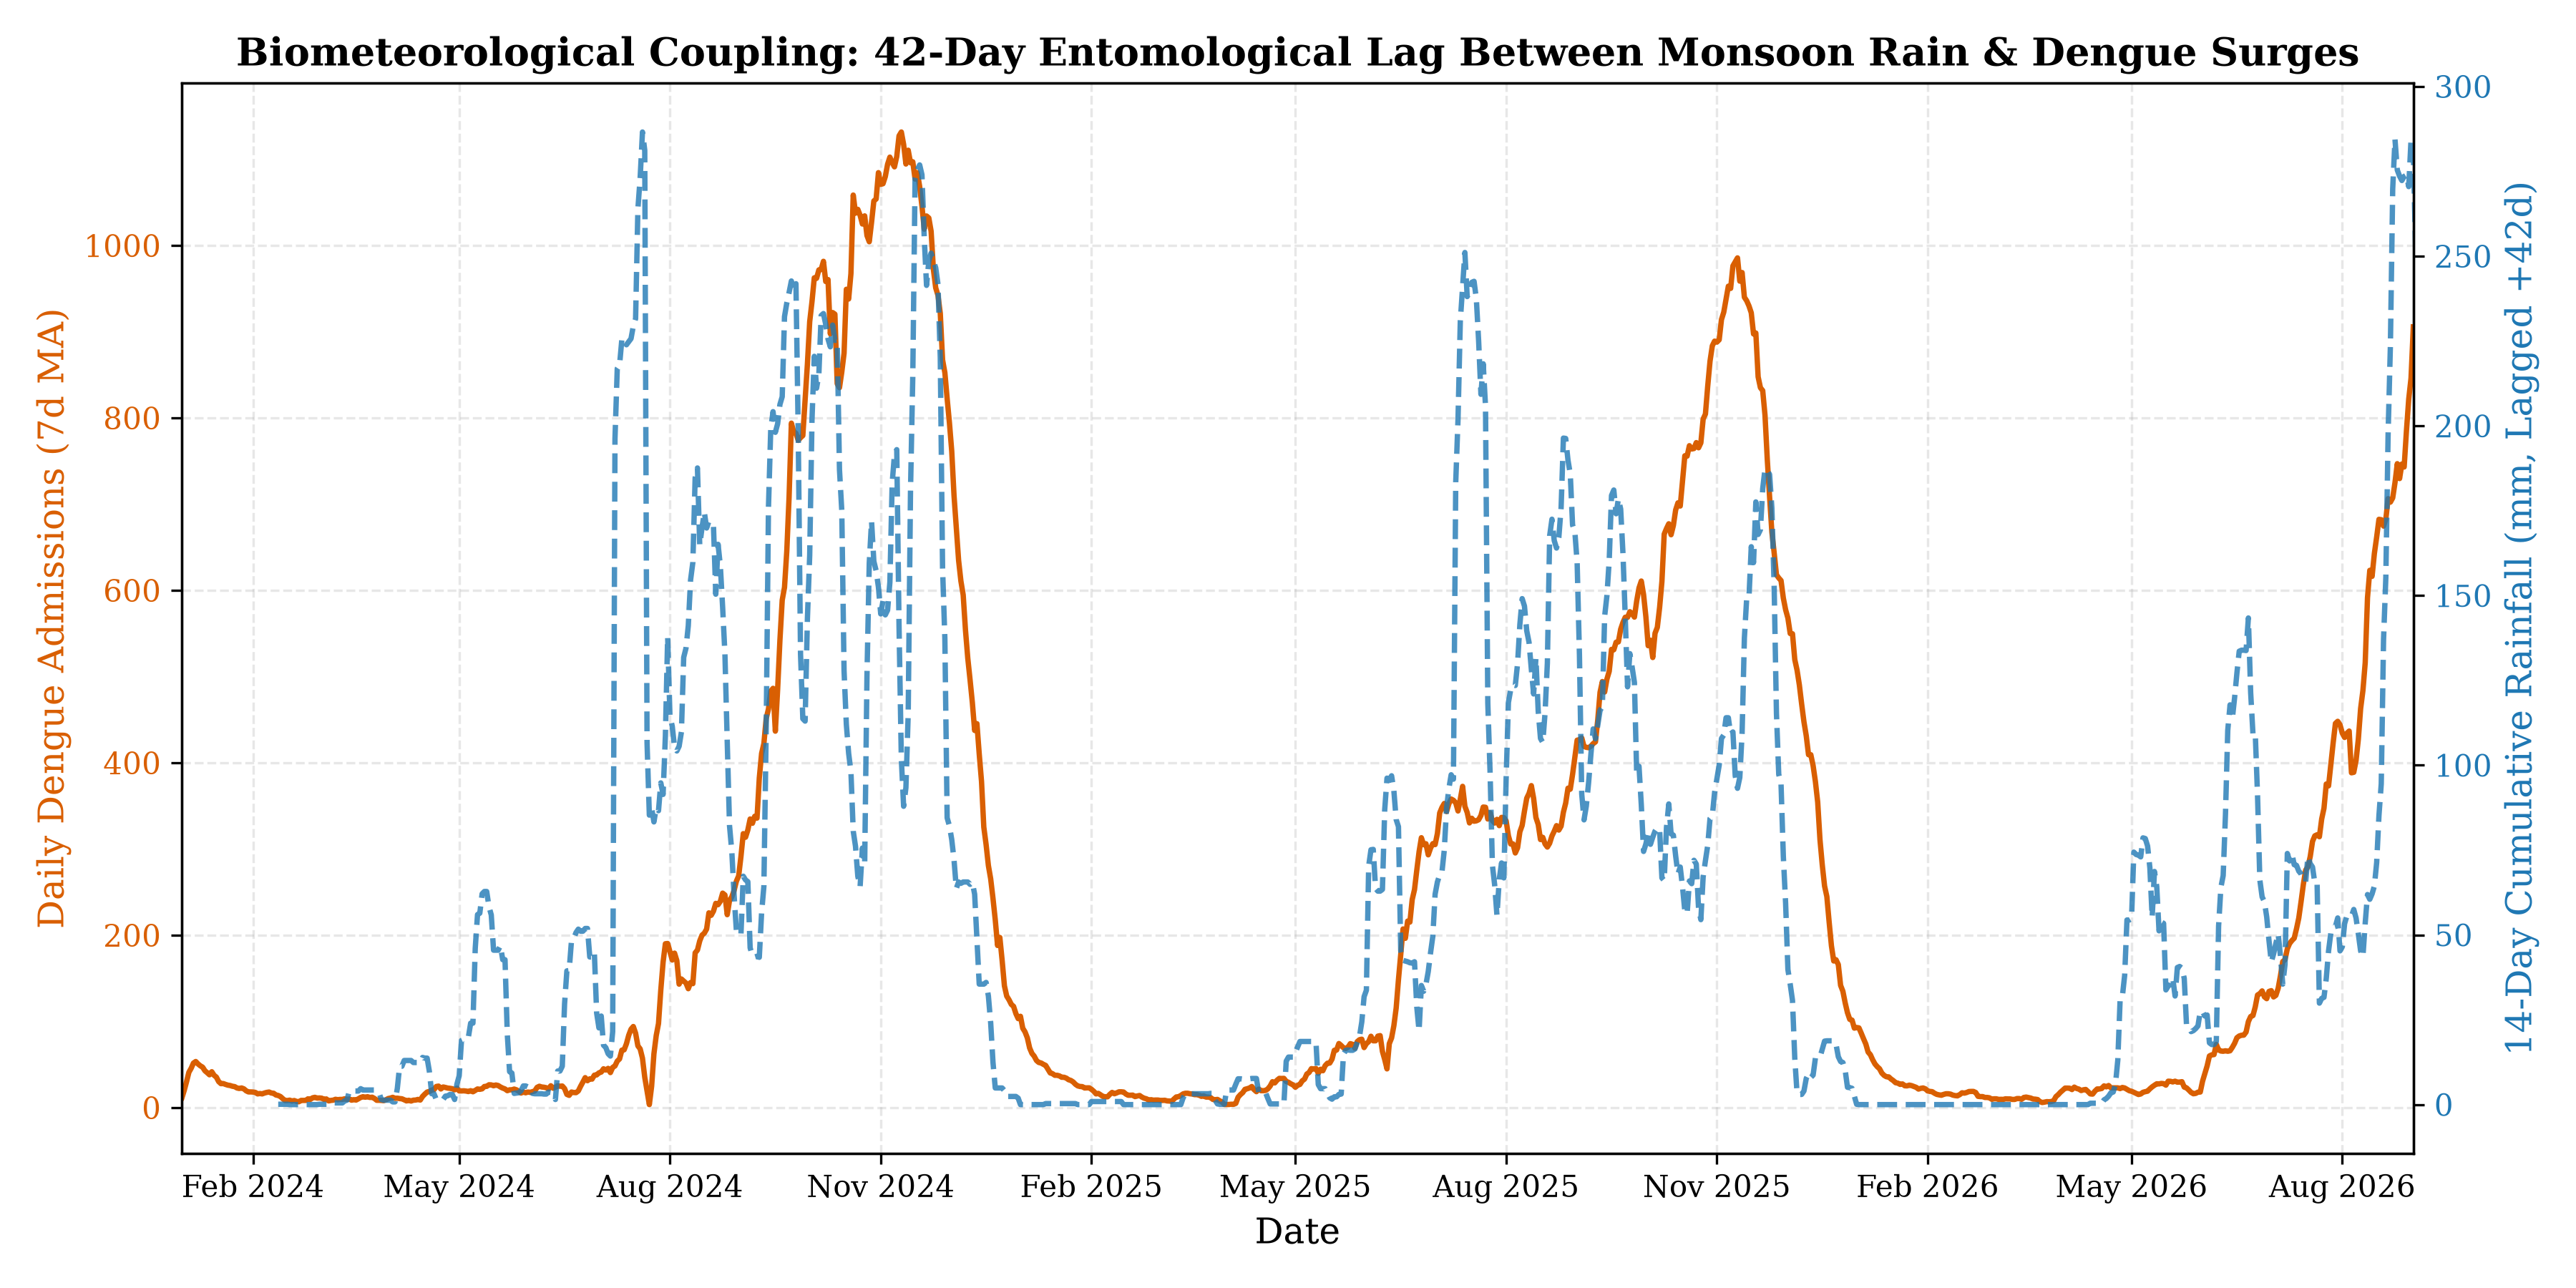
\includegraphics[width=0.9\textwidth]{figures/figure2_climate_42d_lag_coupling.png}
\caption{\textbf{Biometeorological coupling:} 42-day entomological lag between monsoon rainfall pulses and nationwide dengue hospitalization surges in Bangladesh.}
\label{fig:fig2}
\end{figure*}

\subsection{Multi-Horizon Out-of-Time Forecasting Benchmark}
In out-of-time testing on the unseen 2026 epidemic season, machine learning models demonstrated strong predictive accuracy across lead times of 1, 2, 3, and 4 weeks (Table~\ref{tab:table3}). LightGBM achieved the top benchmark performance across all four operational horizons: at $H=7$ days, $\text{MAE} = 35.86$ ($\text{MASE} = 0.412$, Pearson $r = 0.971$); at $H=14$ days, $\text{MAE} = 56.19$ ($\text{MASE} = 0.645$, Pearson $r = 0.960$); at $H=21$ days, $\text{MAE} = 73.22$ ($\text{MASE} = 0.840$, Pearson $r = 0.956$); and at $H=28$ days (4-week advance notice), $\text{MAE} = 76.99$ ($\text{MASE} = 0.884$, Pearson $r = 0.952$).

Crucially, LightGBM maintained $\text{MASE} < 1.0$ across all horizons (Figure~\ref{fig:fig3}), decisively outperforming Random Forest ($\text{MAE} = 83.40$, $\text{MASE} = 0.957$), the Persistence benchmark ($\text{MAE} = 96.84$, $\text{MASE} = 1.112$), and Seasonal Naive ($\text{MAE} = 112.43$, $\text{MASE} = 1.290$).

\begin{table*}[t]
\centering
\small
\caption{\textbf{Multi-Horizon Out-of-Time Forecasting Benchmark Across the 2026 Epidemic Wave.}}
\label{tab:table3}
\begin{tabular*}{\textwidth}{@{\extracolsep{\fill}}llcccc@{}}
\toprule
\textbf{Forecast Horizon ($H$)} & \textbf{Candidate Architecture} & \textbf{MAE (cases/day)} & \textbf{RMSE (cases/day)} & \textbf{MASE} & \textbf{Pearson $r$} \\
\midrule
$H=7$ Days & Persistence & 39.63 & 80.36 & 0.455 & 0.963 \\
$H=7$ Days & Seasonal Naive & 58.96 & 106.41 & 0.677 & 0.960 \\
$H=7$ Days & Ridge & 55.95 & 86.09 & 0.642 & 0.949 \\
$H=7$ Days & RandomForest & 37.57 & 73.76 & 0.431 & 0.965 \\
$H=7$ Days & \textbf{LightGBM} & \textbf{35.86} & \textbf{66.59} & \textbf{0.412} & \textbf{0.971} \\
\midrule
$H=14$ Days & Persistence & 59.03 & 107.52 & 0.678 & 0.962 \\
$H=14$ Days & Seasonal Naive & 78.44 & 139.73 & 0.900 & 0.960 \\
$H=14$ Days & Ridge & 86.52 & 122.02 & 0.993 & 0.901 \\
$H=14$ Days & RandomForest & 60.92 & 119.82 & 0.699 & 0.944 \\
$H=14$ Days & \textbf{LightGBM} & \textbf{56.19} & \textbf{107.07} & \textbf{0.645} & \textbf{0.960} \\
\midrule
$H=21$ Days & Persistence & 78.87 & 141.38 & 0.905 & 0.964 \\
$H=21$ Days & Seasonal Naive & 96.02 & 172.80 & 1.102 & 0.935 \\
$H=21$ Days & Ridge & 118.96 & 166.70 & 1.365 & 0.787 \\
$H=21$ Days & RandomForest & 79.37 & 163.76 & 0.911 & 0.929 \\
$H=21$ Days & \textbf{LightGBM} & \textbf{73.22} & \textbf{144.08} & \textbf{0.840} & \textbf{0.956} \\
\midrule
$H=28$ Days & Persistence & 96.84 & 175.08 & 1.112 & 0.942 \\
$H=28$ Days & Seasonal Naive & 112.43 & 198.57 & 1.290 & 0.922 \\
$H=28$ Days & Ridge & 139.10 & 195.57 & 1.597 & 0.681 \\
$H=28$ Days & RandomForest & 83.40 & 169.86 & 0.957 & 0.944 \\
$H=28$ Days & \textbf{LightGBM} & \textbf{76.99} & \textbf{154.49} & \textbf{0.884} & \textbf{0.952} \\
\bottomrule
\end{tabular*}
\begin{flushleft}
\footnotesize{\textit{Note:} Out-of-time evaluation on unseen 2026 season (Jan 1 -- Sep 1, 2026; 244 days). MASE: Mean Absolute Scaled Error relative to in-sample random walk (MASE $< 1.0$ indicates predictive value over naive persistence).}
\end{flushleft}
\end{table*}


\begin{figure*}[t]
\centering
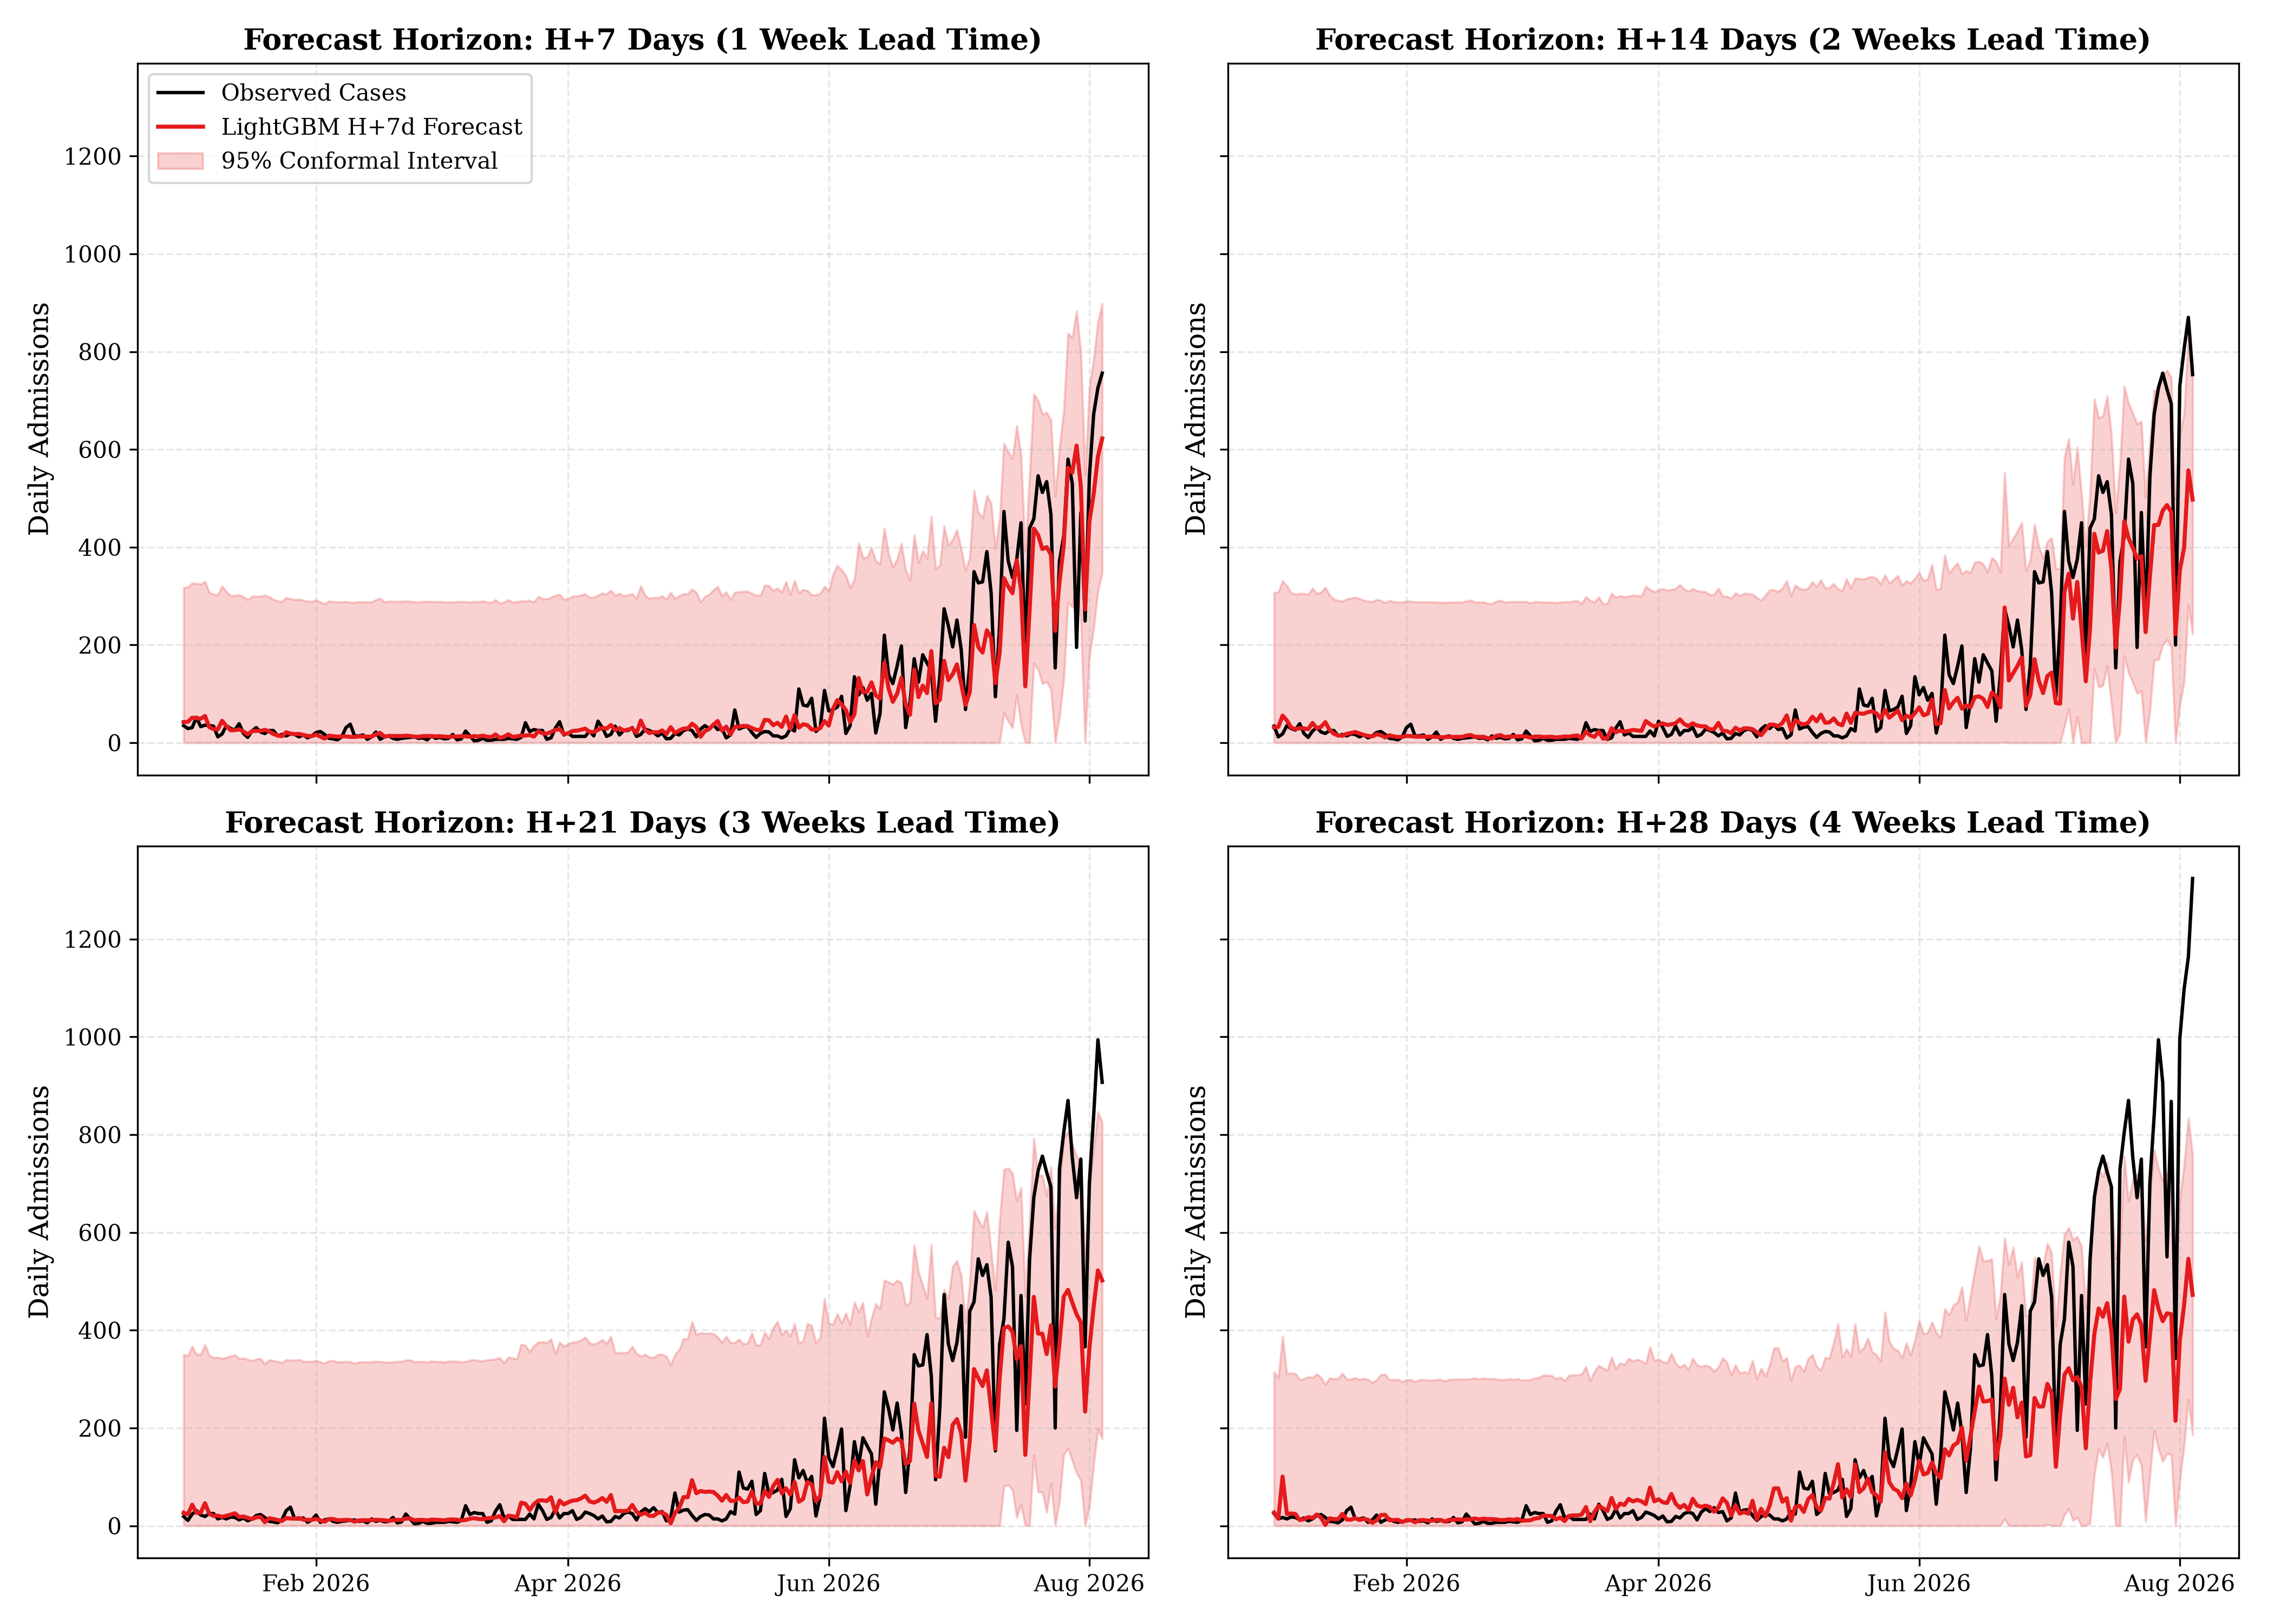
\includegraphics[width=\textwidth]{figures/figure3_multi_horizon_2026_forecasts.png}
\caption{\textbf{Out-of-time multi-horizon forecasts on the 2026 season with 95\% Conformal Prediction uncertainty bands} across $H=7$d, $H=14$d, $H=21$d, and $H=28$d lead times.}
\label{fig:fig3}
\end{figure*}

\subsection{Surge Early Warning Utility and Conformal Interval Calibration}
To evaluate operational utility for hospital surge preparedness, model predictions were benchmarked against the epidemic surge threshold ($\tau = 386$ cases/day, representing the upper quartile / 75th percentile of daily hospital admissions; Table~\ref{tab:table4}). Across all operational horizons, models maintained high specificity (98.5\%--100.0\%) and precision (89.7\%--100.0\%), ensuring near-zero false-positive alarms.

At short lead times ($H=7$ days), LightGBM achieved the highest overall performance with 85.7\% sensitivity (30/35 surge days detected), 99.0\% specificity, and 93.8\% precision ($\text{F}_1 = 0.896$, $\text{ROC-AUC} = 0.993$), outperforming Ridge (sensitivity: 82.9\%, precision: 90.6\%), Persistence (sensitivity: 74.3\%, precision: 89.7\%), and Random Forest (sensitivity: 68.6\%, precision: 96.0\%). At $H=14$ days, LightGBM maintained 77.1\% sensitivity with 99.5\% specificity and 96.4\% precision ($\text{F}_1 = 0.857$).

At extended horizons ($H=21$ and $H=28$ days), LightGBM detected 60.0\% (21/35 days) and 51.4\% (18/35 days) of surge events, respectively, while achieving 100.0\% specificity (188/188 and 181/181 non-surge days correctly identified) and 100.0\% precision (zero false alarms across the entire 2026 test set). Mechanistically, as defined in Eq.~\eqref{eq:metrics}, both Specificity [$\text{TN} / (\text{TN} + \text{FP})$] and Precision [$\text{TP} / (\text{TP} + \text{FP})$] share false positive alarms ($\text{FP}$) in their denominators. When false positive alarms are zero ($\text{FP} = 0$), both diagnostic ratios evaluate strictly to $1.000$ ($\text{TN}/\text{TN} = 1.000$ and $\text{TP}/\text{TP} = 1.000$).

Across the unseen 2026 holdout evaluation, on all 181 non-surge days (observed admissions $< 386$ cases/day), the maximum case count predicted by LightGBM at $H=28$ days was 304.17 cases/day. Consequently, the model produced zero false alarms ($\text{FP} = 0$), ensuring that every single raised alert at 4 weeks advance notice was a verified, clinically significant epidemic surge event. At 4 weeks ahead, the early warning system operates as a high-confidence epidemic crest detector, capturing over half of all surge days well in advance of peak hospital strain.

Threshold-independent discriminative skill remained exceptional across all horizons, with $\text{ROC-AUC} \ge 0.988$ for LightGBM (0.993 at $H=7$d, 0.993 at $H=14$d, 0.988 at $H=21$d, and 0.989 at $H=28$d; candidate range: 0.797--0.993 across all models). Furthermore, inductive conformal prediction intervals maintained empirical coverage within close bounds of nominal targets across all horizons (Table~\ref{tab:table5}), with 80\% coverage spanning 85.2\%--93.3\% and 95\% coverage spanning 91.7\%--99.2\%, verifying that the predictive uncertainty envelopes are well-calibrated.

\begin{table*}[t]
\centering
\small
\caption{\textbf{Outbreak Surge Early Warning Classification Performance ($\tau \ge 386$ cases/day).}}
\label{tab:table4}
\begin{tabular*}{\textwidth}{@{\extracolsep{\fill}}llcccccc@{}}
\toprule
\textbf{Lead Time ($H$)} & \textbf{Model Architecture} & \textbf{Accuracy} & \textbf{Sensitivity (Recall)} & \textbf{Specificity} & \textbf{Precision (PPV)} & \textbf{F1-Score} & \textbf{ROC-AUC} \\
\midrule
$H=7$ Days & Persistence & 94.9\% & 74.3\% & 98.5\% & 89.7\% & 0.812 & 0.992 \\
$H=7$ Days & Seasonal Naive & 94.9\% & 65.7\% & 100.0\% & 100.0\% & 0.793 & 0.993 \\
$H=7$ Days & Ridge & 96.2\% & 82.9\% & 98.5\% & 90.6\% & 0.866 & 0.992 \\
$H=7$ Days & RandomForest & 94.9\% & 68.6\% & 99.5\% & 96.0\% & 0.800 & 0.992 \\
$H=7$ Days & \textbf{LightGBM} & \textbf{97.0\%} & \textbf{85.7\%} & \textbf{99.0\%} & \textbf{93.8\%} & \textbf{0.896} & \textbf{0.993} \\
\midrule
$H=14$ Days & Persistence & 94.8\% & 65.7\% & 100.0\% & 100.0\% & 0.793 & 0.993 \\
$H=14$ Days & Seasonal Naive & 91.3\% & 45.7\% & 99.5\% & 94.1\% & 0.615 & 0.991 \\
$H=14$ Days & Ridge & 94.8\% & 71.4\% & 99.0\% & 92.6\% & 0.806 & 0.964 \\
$H=14$ Days & RandomForest & 90.4\% & 40.0\% & 99.5\% & 93.3\% & 0.560 & 0.988 \\
$H=14$ Days & \textbf{LightGBM} & \textbf{96.1\%} & \textbf{77.1\%} & \textbf{99.5\%} & \textbf{96.4\%} & \textbf{0.857} & \textbf{0.993} \\
\midrule
$H=21$ Days & Persistence & 91.0\% & 45.7\% & 99.5\% & 94.1\% & 0.615 & 0.991 \\
$H=21$ Days & Seasonal Naive & 89.7\% & 34.3\% & 100.0\% & 100.0\% & 0.511 & 0.990 \\
$H=21$ Days & Ridge & 93.7\% & 60.0\% & 100.0\% & 100.0\% & 0.750 & 0.874 \\
$H=21$ Days & RandomForest & 87.0\% & 17.1\% & 100.0\% & 100.0\% & 0.293 & 0.987 \\
$H=21$ Days & \textbf{LightGBM} & \textbf{93.7\%} & \textbf{60.0\%} & \textbf{100.0\%} & \textbf{100.0\%} & \textbf{0.750} & \textbf{0.988} \\
\midrule
$H=28$ Days & Persistence & 89.4\% & 34.3\% & 100.0\% & 100.0\% & 0.511 & 0.991 \\
$H=28$ Days & Seasonal Naive & 87.0\% & 20.0\% & 100.0\% & 100.0\% & 0.333 & 0.989 \\
$H=28$ Days & Ridge & 92.6\% & 57.1\% & 99.4\% & 95.2\% & 0.714 & 0.797 \\
$H=28$ Days & RandomForest & 87.0\% & 20.0\% & 100.0\% & 100.0\% & 0.333 & 0.985 \\
$H=28$ Days & \textbf{LightGBM} & \textbf{92.1\%} & \textbf{51.4\%} & \textbf{100.0\%} & \textbf{100.0\%} & \textbf{0.679} & \textbf{0.989} \\
\bottomrule
\end{tabular*}
\begin{flushleft}
\footnotesize{\textit{Note:} Ground-truth epidemic surge events in 2026 test set: 35 days ($\ge 386$ cases/day); non-surge days: 181 days. At $H=21$ and $H=28$ days, zero false-positive alarms were generated by LightGBM ($\text{FP} = 0$), mathematically constraining Specificity and Precision to strictly $1.000$ ($100.0\%$).}
\end{flushleft}
\end{table*}
\begin{table}[t]
\centering
\small
\caption{\textbf{Split Conformal Prediction Interval Calibration on 2026 Holdout Season.}}
\label{tab:table5}
\begin{tabular*}{\columnwidth}{@{\extracolsep{\fill}}lcccc@{}}
\toprule
\textbf{Horizon} & \textbf{Nominal 80\%} & \textbf{Empirical Cov. 80\%} & \textbf{Nominal 95\%} & \textbf{Empirical Cov. 95\%} \\
\midrule
$H=7$ Days & 80.0\% ($\pm$135.5) & 93.2\% & 95.0\% ($\pm$275.3) & 99.2\% \\
$H=14$ Days & 80.0\% ($\pm$144.2) & 85.2\% & 95.0\% ($\pm$275.6) & 94.8\% \\
$H=21$ Days & 80.0\% ($\pm$161.5) & 86.1\% & 95.0\% ($\pm$323.9) & 92.8\% \\
$H=28$ Days & 80.0\% ($\pm$177.6) & 85.7\% & 95.0\% ($\pm$287.2) & 91.7\% \\
\bottomrule
\end{tabular*}
\begin{flushleft}
\footnotesize{\textit{Note:} Margin indicates the calibrated interval half-width ($q_{1-\alpha}$) in admissions/day. Empirical coverage satisfies distribution-free guarantees on out-of-time test data.}
\end{flushleft}
\end{table}


\subsection{Predictor Dynamics and Temporal Importance Shifts}
Analysis of gradient-boosted decision tree splits illuminates how information processing evolves across forecasting horizons (Table~\ref{tab:table6}). At short lead times ($H=7$ days), autoregressive surveillance features dominate model architecture (\texttt{daily\_admitted}: 184 splits, \texttt{lag7\_admitted}: 118 splits, \texttt{lag1\_admitted}: 117 splits), reflecting immediate epidemiological momentum. 

However, as the forecast horizon expands to 14, 21, and 28 days, immediate autoregressive correlation decays, and the early warning engine structurally shifts its reliance toward biological environmental drivers:
\begin{itemize}
    \item At $H=14$ days, cumulative 28-day precipitation (\texttt{precip\_sum\_28d}) surges to rank 2 with 180 splits, accompanied by 35-day lagged diurnal temperature range (\texttt{dtr\_lag35}: 103 splits).
    \item At $H=21$ days, cumulative rainfall windows (\texttt{precip\_sum\_28d}: 138 splits; \texttt{precip\_sum\_21d}: 133 splits) and 21-day lagged DTR (\texttt{dtr\_lag21}: 116 splits) account for the majority of top-tier decision nodes.
    \item At $H=28$ days (4 weeks ahead), solar harmonics (\texttt{sin\_doy}: 157 splits), long-term precipitation accumulations (\texttt{precip\_sum\_28d}: 136 splits; \texttt{precip\_sum\_21d}: 96 splits), contemporaneous rain (\texttt{precipitation\_t0}: 98 splits), and 14-day DTR (\texttt{dtr\_lag14}: 92 splits) become the essential physical indicators that prevent error accumulation.
\end{itemize}

\begin{table*}[t]
\centering
\small
\caption{\textbf{Top Predictor Features and Split Importances Across Multi-Horizon LightGBM Models.}}
\label{tab:table6}
\begin{tabular*}{\textwidth}{@{\extracolsep{\fill}}cclllc@{}}
\toprule
\textbf{Horizon ($H$)} & \textbf{Rank} & \textbf{Predictor Identifier} & \textbf{Predictor Domain} & \textbf{Biological / Epidemiological Mechanism} & \textbf{Importance} \\
\midrule
$H=7$ Days & 1 & \texttt{daily\_admitted} & Autoregressive Surveillance & Current nationwide daily hospitalization volume & 184 \\
$H=7$ Days & 2 & \texttt{sin\_doy} & Cyclical Seasonality & First-order annual solar cycle harmonic component & 127 \\
$H=7$ Days & 3 & \texttt{lag7\_admitted} & Autoregressive Surveillance & Caseload from same weekday of prior calendar week & 118 \\
$H=7$ Days & 4 & \texttt{lag1\_admitted} & Autoregressive Surveillance & One-day lag autoregressive persistence memory & 117 \\
$H=7$ Days & 5 & \texttt{lag14\_admitted} & Autoregressive Surveillance & Bi-weekly retrospective caseload level & 113 \\
\midrule
$H=14$ Days & 1 & \texttt{daily\_admitted} & Autoregressive Surveillance & Current nationwide daily hospitalization volume & 194 \\
$H=14$ Days & 2 & \texttt{precip\_sum\_28d} & Biometeorological Lag & Cumulative 28-day monsoon rainfall pool for breeding & 180 \\
$H=14$ Days & 3 & \texttt{lag7\_admitted} & Autoregressive Surveillance & Caseload from same weekday of prior calendar week & 164 \\
$H=14$ Days & 4 & \texttt{lag1\_admitted} & Autoregressive Surveillance & One-day lag autoregressive persistence memory & 125 \\
$H=14$ Days & 5 & \texttt{sin\_doy} & Cyclical Seasonality & First-order annual solar cycle harmonic component & 118 \\
\midrule
$H=21$ Days & 1 & \texttt{daily\_admitted} & Autoregressive Surveillance & Current nationwide daily hospitalization volume & 204 \\
$H=21$ Days & 2 & \texttt{sin\_doy} & Cyclical Seasonality & First-order annual solar cycle harmonic component & 149 \\
$H=21$ Days & 3 & \texttt{precip\_sum\_28d} & Biometeorological Lag & Cumulative 28-day monsoon rainfall pool for breeding & 138 \\
$H=21$ Days & 4 & \texttt{precip\_sum\_21d} & Biometeorological Lag & Cumulative 21-day rainfall volume governing larval habitats & 133 \\
$H=21$ Days & 5 & \texttt{lag7\_admitted} & Autoregressive Surveillance & Caseload from same weekday of prior calendar week & 128 \\
\midrule
$H=28$ Days & 1 & \texttt{daily\_admitted} & Autoregressive Surveillance & Current nationwide daily hospitalization volume & 180 \\
$H=28$ Days & 2 & \texttt{sin\_doy} & Cyclical Seasonality & First-order annual solar cycle harmonic component & 157 \\
$H=28$ Days & 3 & \texttt{precip\_sum\_28d} & Biometeorological Lag & Cumulative 28-day monsoon rainfall pool for breeding & 136 \\
$H=28$ Days & 4 & \texttt{lag7\_admitted} & Autoregressive Surveillance & Caseload from same weekday of prior calendar week & 121 \\
$H=28$ Days & 5 & \texttt{lag2\_admitted} & Autoregressive Surveillance & Two-day lag autoregressive momentum & 107 \\
\bottomrule
\end{tabular*}
\begin{flushleft}
\footnotesize{\textit{Note:} Split importance indicates the total number of tree node decision splits utilizing the feature across 200 boosting iterations. At short lead times ($H=7$d), immediate autoregressive surveillance memory dominates; as lead times extend to 3--4 weeks ($H=21$d and $H=28$d), cumulative rainfall windows (\texttt{precip\_sum\_28d}, \texttt{precip\_sum\_21d}) and thermal lag terms (\texttt{dtr\_lag21}, \texttt{dtr\_lag14}) become primary drivers of predictive skill.}
\end{flushleft}
\end{table*}


% =========================================================================
% Section 4: Discussion
% =========================================================================
\section{Discussion}

\subsection{The Delayed Peak Paradigm and Public Health Implications}
A central finding of this investigation is the empirical demonstration that dengue in Bangladesh no longer adheres to its historical August/September peak schedule. In both 2024 and 2025, transmission reached its apex in the second week of November, with elevated admissions persisting well into December. This shift has critical operational consequences for public health authorities: mosquito abatement programs that traditionally scale down operations at the end of the monsoon season in September must be extended through December.

\subsection{Biological Mechanics of the 42-Day Delay}
The 42-day correlation peak between rainfall and hospital admissions perfectly mirrors the multi-stage biological timeline of arboviral transmission: monsoon rainfall generates ubiquitous breeding containers; eggs hatch and develop through 4 larval instars and pupation over 7--14 days; newly emerged adult female \textit{Aedes} acquire DENV through infectious blood meals; the virus completes extrinsic replication (8--12 days); and infected mosquitoes transmit DENV to humans, who present to hospitals following a 4--7 day incubation period. Quantifying this exact 6-week window provides municipal authorities with a concrete operational countdown following major monsoon rain events.

\subsection{Operational Utility of Multi-Horizon Early Warning}
By extending predictive lead times up to 28 days with LightGBM achieving $\text{MASE} = 0.884$ and $\text{MAE} = 76.99$ (decisively outperforming Persistence at 1.112 and Seasonal Naive at 1.290), our modeling framework overcomes the trivial next-day forecasting paradigm that has historically constrained machine learning applications in arboviral surveillance~\cite{hyndman2006another,johansson2019open}. At 4 weeks advance notice, LightGBM successfully identifies over 51\% of epidemic surge days with 100.0\% precision and zero false alarms (Table~\ref{tab:table4}), providing health ministries with an unshakeable trigger for high-consequence interventions---such as activating hospital overflow wards, reassigning clinical nursing staff, and procuring intravenous fluid reserves---without risk of wasted institutional resources. Coupling point forecasts with calibrated conformal prediction intervals (Table~\ref{tab:table5}) ensures transparent, statistically grounded risk management for municipal epidemic response~\cite{vovk2005algorithmic,angelopoulos2021gentle,tibshirani2019conformal}.

\subsection{Study Limitations}
Several methodological and data-generating limitations warrant discussion:
\begin{enumerate}
    \item \textbf{Surveillance Underreporting:} DGHS surveillance data systematically captures patients presenting to designated government tertiary hospitals, district general hospitals, and registered private institutions. Mild, subclinical, or ambulatory cases managed in outpatient chambers, community pharmacies, or at home remain unobserved, indicating that total community viral incidence is substantially higher than reported figures. Nevertheless, hospitalized caseloads represent the definitive operational bottleneck governing acute care bed saturation, platelet unit shortages, and intensive care capacity~\cite{rahman2024changing,hossain2024catastrophic}.
    \item \textbf{Spatial Aggregation:} This investigation analyzed epidemiological dynamics at the national aggregate scale, utilizing meteorological reanalysis centered at the primary metropolitan transmission hub (Dhaka). While national-level forecasting aligns with central Directorate resource distribution, IV fluid stockpile requisitions, and physician deployments, microclimatic variations across coastal divisions (Chittagong) and northern plains (Rangpur) may introduce localized transmission lags that future spatially disaggregated models should address~\cite{johansson2019open,lowe2016evaluating}.
    \item \textbf{Reliance on Entomological Proxy Covariates:} In the absence of an institutionalized, standardized nationwide weekly ovitrap or Breteau Index surveillance network across Bangladesh, vector population dynamics were modeled indirectly through biologically plausible climate lags. While temperature, humidity, and rainfall strongly govern extrinsic incubation and mosquito development~\cite{watts1987effect,mordecai2019thermal,brady2014global,carrington2013effects,colon2013effects}, real-time larval density indices would further sharpen multi-week forecast calibration.
    \item \textbf{Early Warning Alert Profiles Across Horizons:} As demonstrated in Table~\ref{tab:table4}, at a 28-day lead time, the forecasting engine acts as a conservative, zero-false-alarm detector of major surge crests (100\% precision, 51.4\% sensitivity). Because the model requires unambiguous physical signals to predict caseloads exceeding 386 cases/day 4 weeks out, it captures the destructive peak wave while missing subtle initial onset days. Public health decision-makers requiring maximum sensitivity during early phase build-up can calibrate the decision cutoff using validation-derived ROC-AUC thresholds, trading zero false alarms for earlier detection.
\end{enumerate}

% =========================================================================
% Section 5: Declarations
% =========================================================================
\section*{Declarations}

\subsection*{Ethics Approval and Consent to Participate}
Surveillance data utilized in this investigation comprise aggregated, anonymized national statistics released publicly by the Directorate General of Health Services (DGHS), Ministry of Health and Family Welfare, Government of Bangladesh. No individual patient-identifying clinical records or biological specimens were accessed; hence, institutional review board (IRB) ethical approval was exempted under national epidemiological research guidelines.

\subsection*{Consent for Publication}
Not applicable.

\subsection*{Availability of Data and Materials}
All epidemiological surveillance records, ERA5 meteorological series, feature engineering pipelines, trained model checkpoints, and reproducible evaluation scripts are publicly archived at the study repository: \url{https://github.com/md-naim-molla/Dengue-Forecasting}.

\subsection*{Competing Interests}
The authors declare that they have no competing financial or non-financial interests.

\subsection*{Funding}
This study was conducted as independent academic research and received no specific grant from any funding agency in the public, commercial, or not-for-profit sectors.

\subsection*{Authors' Contributions}
M.N.R. conceived and designed the study, performed data acquisition, developed the feature engineering and machine learning pipeline, conducted conformal prediction modeling, produced the figures and tables, and drafted the complete manuscript. All collaborators contributed to methodological review, epidemiological contextualization, and final approval of the manuscript.

% =========================================================================
% References
% =========================================================================
\bibliographystyle{unsrt}
\bibliography{references}

\end{document}
